% fixture: tikz/calc-pdftex
% oracle: pdflatex
% tier: T3
% engine: document
% specials: compare
% covers: calc's coordinates (sums, factors, partway, distance and projection modifiers, rotation, between nodes' anchors, with coordinate options); x= and y= as lengths and as points (pgfpointxy everywhere: coordinates, circles, arcs, grids, positioning's distances); scale with a vector; line cap, line join, miter limit; opacity, fill opacity, draw opacity and the transparency styles
% issue: #326
\documentclass{article}
\usepackage{tikz}
\usetikzlibrary{calc,positioning}
\begin{document}
\noindent Calc: 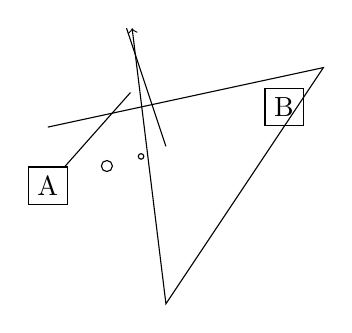
\begin{tikzpicture}
  \node[draw] (a) {A};
  \node[draw] (b) at (3,1) {B};
  \draw ($(a)!.25!(b)$) circle (2pt) ($(a.east)!1cm!(b.west)$) circle (1pt);
  \draw ($(a)!(1,2)!(b)$) -- (1,2) ($(a)!0.5!30:(b)$) -- (a);
  \draw[->] ($(a.north)+(0,0.5)$) -- ($(b)+.5*(1,1)$) -- ($2*(1,0)-(0,1)-.5*(1,1)$) -- ([xshift=2pt]$(1,1)+(0,1)$);
\end{tikzpicture}

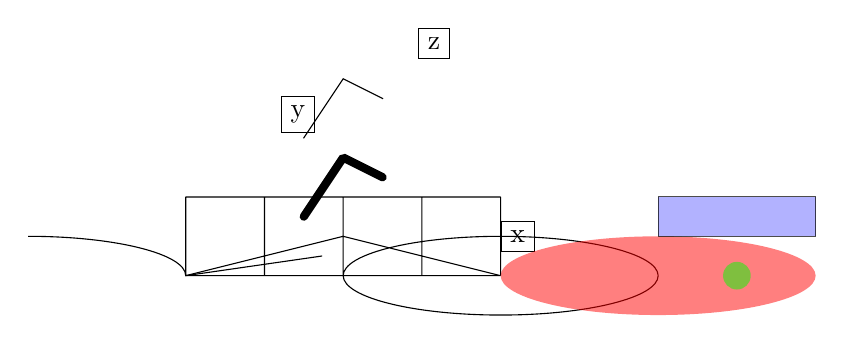
\begin{tikzpicture}[x=2cm,y=0.5cm]
  \draw (0,0) -- (1,1) -- (2,0) circle (1) (0,0) grid (2,2);
  \draw (30:1) -- (0,0) arc (0:90:1);
  \node[draw,right=1 of {(1,1)}] {x};
  \begin{scope}[x={(1cm,0.5cm)},y={(0cm,1cm)},scale=0.5]
    \draw[line cap=round,line join=bevel,line width=3pt] (3,0) -- (4,1) -- (5,0);
    \draw[line cap=rect,miter limit=4] (3,2) -- (4,3) -- (5,2);
    \node[draw,above right=1 of {(1,1)}] {y};
    \node[draw,y={(0.3cm,1cm)},above right=1 and 2 of {(1,1)}] {z};
  \end{scope}
  \fill[red,opacity=0.5] (3,0) circle (1);
  \filldraw[fill=blue,fill opacity=0.3,draw opacity=0.7] (3,1) rectangle (4,2);
  \fill[semitransparent,green] (3.5,0) circle (5pt);
\end{tikzpicture}
\end{document}
